\section{Methodology}
Assuming that $X_j$ is in the domain of attraction of a max stable distribution
  for each $j$, then the standardization of $X$ to GPD process occurs as follows:

\begin{equation}
Z_{j} = \left(1 + \gamma_j\frac{X_{j} - b_{tj}}{a_{tj}}\right)_{+}^{1/\gamma_j}
\end{equation}
where $b_{tj} = F^{-1}(1-1/t)$, and $a_{tj}$ and $\gamma_{j}$ are evaluated via
  maximum likelihood \makenote{(need to fix)}.  The quantity
  $\left(1 + \gamma_j\frac{X_{j} - b_{tj}}{a_{tj}}\right)_+$ is left truncated
  at 0.  Note that $Z_j > 1$ indicates that $X_{j} > b_{tj}$, meaning that the
  observation was \emph{extreme} in that dimension.  Recognize here that $Z_i$
  exists on the positive orthant in Euclidean space, $\mathcal{R}_+^d$, and
  that $\max_jZ_j$ follows a simple Pareto distribution.  Additionally, we can
  transform ${\bf Z} \rightarrow (R, {\bf V})$, where:
\begin{equation}
  \begin{aligned}
    R &= \lVert {\bf z} \rVert_{\infty} = \max_{j \in (1,\ldots,d)} z_i\\
    {\bf V} &= \left(\frac{z_1}{R},\ldots,\frac{z_d}{R}\right) \in S_{\infty}^{d-1}.\\
  \end{aligned}
\end{equation}

Thus ${\bf V}$ is the projection of the ${\bf Z}$ vector onto the unit
  hypersphere, using the $L_{\infty}$ norm.  As stated before by homogeneity
  property, a spectral measure $\Phi$ on some space in $S_{\infty}^{d-1}$ is
  independent of $R$, which follows the standard Pareto distribution by
  construction.

We are interested in the angular distribution of ${\bf V}$, the projection of
  the standardized observations ${\bf Z}$ onto the unit hypersphere. To
  construct a parametric model on that angular distribution, we employ the
  projected gamma distribution.

\subsection{Projected Gamma}
\label{method:pg}
The projected gamma distribution, developed in \cite{nunez2019}, is built upon
  the product of $d$ independent gamma distributions.  That is, for
  ${\bf y} = (y_1,\ldots,y_d)^t$, and $y_i\sim\text{Ga}(\alpha_i,\beta_i)$, we
  define our starting point:
\begin{equation}
    f({\bf y}\mid{\bf \alpha},{\bf \beta}) = \prod_{j = 1}^d\text{Ga}(y_j\mid\alpha_j,\beta_j),
\end{equation}
where $\beta$ is specified as a rate parameter.  From that, we transform to
  $d$-dimensional spherical coordinates ${\bf y} \rightarrow (r,{\bf \theta})$
  as
\begin{equation}
  \label{eqn:transform}
  \begin{aligned}
    y_1     &= r\cos\theta_1,\\
    y_2     &= r\sin\theta_1\cos\theta_2\\
            &\vdots\\
    y_{d-1} &= r\sin\theta_1\ldots\sin\theta_{d-2}\\
    y_{d}   &= r\sin\theta_1\ldots\sin\theta_{d-1}
  \end{aligned}
\end{equation}
where $r = \lVert {\bf y}\rVert_{2}$, the euclidean norm of ${\bf y}$.  The
  inverse of this transformation is:
\begin{equation}
  \label{eqn:invtransform}
  \begin{aligned}
    \theta_1     &= \cos^{-1}\left[\frac{y_1}{\lVert y_{1:d}\rVert_2}\right]\\
    \theta_2     &= \cos^{-1}\left[\frac{y_2}{\lVert y_{2:d}\rVert_2}\right]\\
                 &\vdots\\
    \theta_{d-1} &= \cos^{-1}\left[\frac{y_{d-1}}{\lVert y_{(d-1):d}\rVert_2}\right].
  \end{aligned}
\end{equation}
The Jacobian of this transformation is
\begin{equation*}
r^{d-1}\prod_{i = 1}^{d-2}(\sin\theta_i)^{d-1-i}.
\end{equation*}
This creates the distribution over $r,{\bf \theta}$.  The full conditional for
  $r$ takes the form of a Gamma random variable, and we can integrate it out as
  such.  This leaves the \emph{projected gamma distribution},
\begin{equation}
    \text{PG}({\bf \theta}\mid{\bf \alpha},{\bf \beta}) = \frac{\Gamma(A)\beta_d^{\alpha_d}}{B^A\Gamma(a_d}\left(\prod_{j = 1}^{d-1}\frac{\beta_j^{\alpha_j}}{\Gamma(\alpha_j)}(\cos\theta_j)^{\alpha_j - 1}(\sin\theta_j)^{(\sum_{h = j + 1}^d\alpha_h) - 1}\right)\mathcal{I}_{(0,\pi/2)^{d-1}}({\bf \theta})
\end{equation}
where
\begin{equation}
    A = \sum_{j = 1}^d\alpha_j \hspace{1cm}\text{and}\hspace{1cm}B = \beta_1\cos\theta_1 + \sum_{j = 2}^{d-1}\left(\beta_j\cos\theta_j\prod_{i = 1}^{j-1}\sin\theta_i\right) + \beta_d\prod_{j = 1}^d-1\sin\theta_j.
\end{equation}
As is, this model is not identifiable, as taking
  ${\bf \beta}^{(2)} = \alpha {\bf \beta}^{(1)}$ will still yield the same
  distribution of angles. Following \cite{nunez2019}, we have opted to place a
  restriction on $\beta$ such that $\beta_1 := 1$, thus
  ${\bf \beta} = (1, \beta_2, \ldots, \beta_d)^t$.

Inference on this model can take two forms: ${\bf \alpha}$ and ${\bf \beta}$ in
  this form can not be broken down into known-form full conditionals, so we can
  conduct a Metropolis Hastings step for every component, or do a joint proposal
  Metropolis Hastings step for all components at once.  Alternatively, using
  $f(r,{\bf \theta})$, we recognize that $\alpha_i\mid r$ is independent of
  $\alpha_j\mid r$, so we can sample the latent $r$ and conduct independent
  Gibbs steps for each component.  Further, in sampling the $\alpha_j$'s, we can
  integrate out $\beta_j$. Within the Gibbs sampler, we sample $r$, then each
  $\alpha_j\mid r$, then each $\beta_j\mid r, \alpha_j$.  This leads to fast
  convergence, with the only Metropolis Hastings step being for the
  $\alpha_j$'s.  Both $r$ and the $\beta_j$'s are Gamma distributed.

For simplicity, let ${\bf y^{\prime}} = r^{-1}{\bf y}$.  That is,
  ${\bf y^{\prime}}$ is a function of the angular data--from~\eqref{eqn:transform},
  ${\bf y^{\prime}} = {\bf y}/r$, the projection of the ${\bf y}$ vector onto
  the unit hypersphere. We generate a latent $r$, and their product is the
  latent ${\bf y}$.  Given ${\bf y}$, the posterior distributions for
  $(\alpha_i, \beta_i)$, $(\alpha_j,\beta_j)$, $i\neq j$ are independent.

As~\cite{nunez2019} shows, the projected gamma distribution is a flexible model
  for representing data on the positive orthant of the unit hypersphere.  As such,
  given our application restricts us to this domain, one can see that this might be a
  natural choice of distribution for our purpose.

\begin{figure}[h!]
  \centering
  \label{fig:vanillamix}
  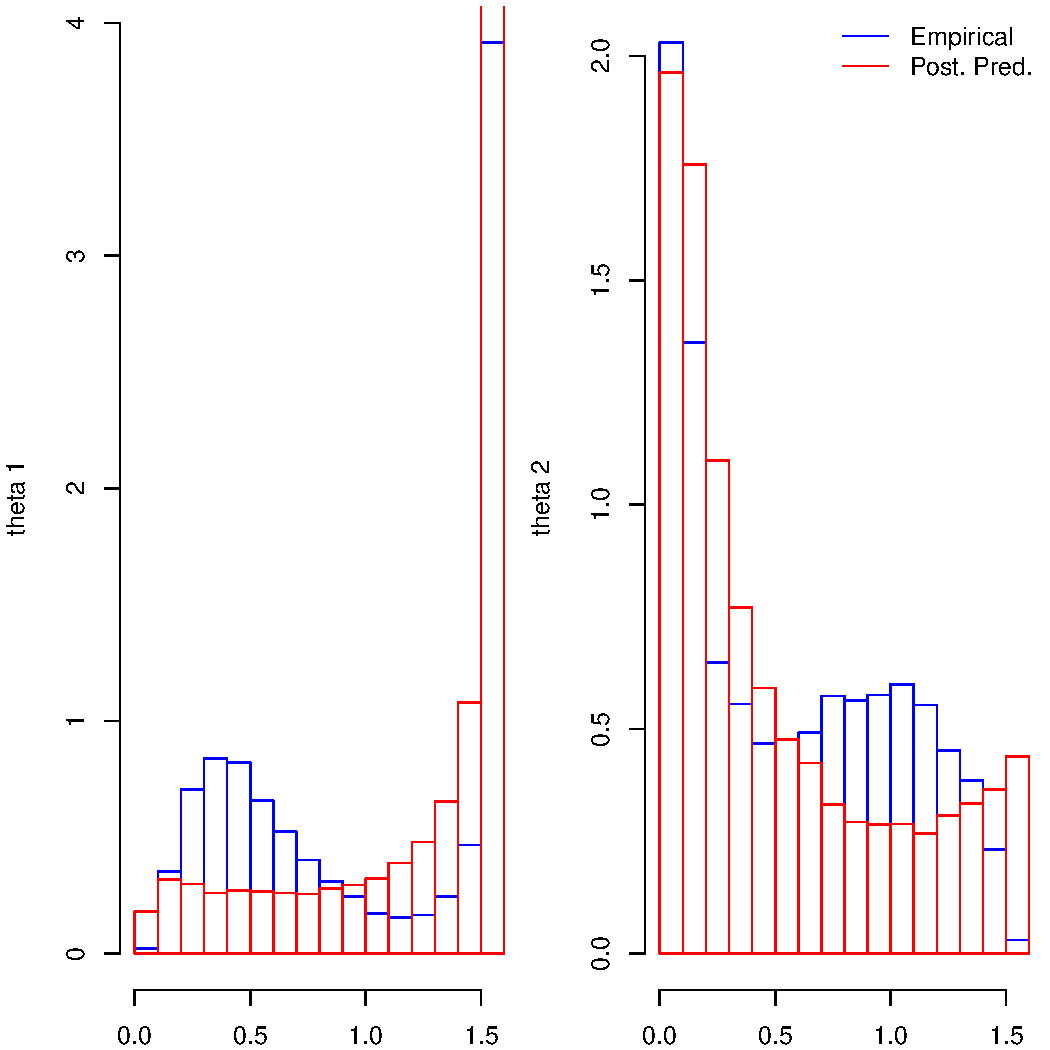
\includegraphics[width=5in]{./images/justification_for_more_complex_models}
  \caption{Histograms of Empirical vs Posterior-predictive angular data originating
            from a simulated 3-dimensional gamma dataset.}
\end{figure}

However, as flexible as it is, it alone is not sufficient for our purpose.  Supposing
  a given dataset is the result of two or more generating distributions, then using a
  a single distribution to represent this dataset becomes untenable.  In Figure~\ref{fig:vanillamix}
  we see the empirical distribution a 2-component mixture of projected gammas, plotted
  against the posterior predictive distribution of a projected gamma model fitted to
  that dataset.  As we can see, it has trouble representing the nuances of the two
  component mixture.


% EOF



\subsection{Projected Mixture of Gammas (PMG) Model}
\label{method:pmg}
One shortcoming of the vanilla method is there could be multiple
  generating distributions for the extreme events.  Indeed, if we attempt to
  model real data and observe the marginal empirical distributions of $\theta$
  versus the marginal predicted, we observe a disconnect: the marginal predicted
  on some axes looks very different from the marginal empirical.  We attempt to
  solve this problem by creating a two-component mixture model for each gamma.

A justification for this model is that, while more complex than the vanilla model,
  it is significantly less complex than the mixtures of projected gamma, whether
  finite or non-finite.  If we can represent the nuances of real data using a more
  parsimonious model, then that would be preferred.

As previously stated, ${\bf y}$ represents a an array of latent gamma variates.
  This model considers each marginal gamma as a 2-component mixture model.
  I.e., ${\bf y} = r{\bf y^{\prime}}$, where ${\bf y^{\prime}}$ is a function of
  the data; considering only the $j$th column of ${\bf y}$, considering only a
  single observation:
\begin{equation*}
  f(y_j\mid {\bf \alpha}_j, {\bf \beta}_j, \lambda_j) = \lambda_j\text{Ga}(y_j\mid\alpha_{j1},\beta_{j1}) + (1 - \lambda_j)\text{Ga}(y_j\mid\alpha_{j2}, \beta_{j2})
\end{equation*}
To make this Gibbs-able, we add a latent flag,
  $\gamma_j \in \lbrace 0, 1\rbrace$ which indicates which part of the mixture
  the observation $y_j$ is coming from.  That is,
\begin{equation*}
f(y_j, \gamma_j \mid{\bf \alpha}_j, {\bf \beta}_j, \lambda_j) = \left(\lambda_j\text{Ga}(y_j\mid\alpha_{j1},\beta_{j1})\right)^{\gamma_j}\left((1-\lambda_j)\text{Ga}(y_j\mid\alpha_{j2},\beta_{j2})\right)^{1-\gamma_j}
\end{equation*}
Then, considering the likelihood of ${\bf y}_j$:
\begin{equation*}
  \begin{aligned}
    L({\bf y}_j,{\bf \gamma}_j\mid{\bf\alpha}_j,{\bf \beta}_j, \lambda_j) &= \prod_{i = 1}^n\left(\lambda_j\text{Ga}(y_{ij}\mid\alpha_{j1},\beta_{j1})\right)^{\gamma_{ij}}\left((1-\lambda_j)\text{Ga}(y_{ij}\mid\alpha_{j2},\beta_{j2})\right)^{1-\gamma_{ij}}\\
    &= \frac{(\lambda_j)^{n_j}\beta_{j,1}^{\alpha_{j,1}n_{j}}}{\Gamma(\alpha_{j,1})^{n_{j}}}\left(\prod_{i:\gamma_{ij} = 1}y_{ij}\right)^{\alpha_{j1} - 1}\exp\left\lbrace-\beta_{j1}\sum_{i:\gamma_{ij} = 1}y_{ij}\right\rbrace\\
    &\hspace{0.5cm}\times\frac{(1 - \lambda_j)^{n - n_j}\beta_{j2}^{\alpha_{j2}(n - n_j)}}{\Gamma(\alpha_{j2})^{n - n_j}}\left(\prod_{i:\gamma_{ij} \neq 1}y_{ij}\right)^{\alpha_{j2} - 1}\exp\left\lbrace-\beta_{j2}\sum_{i:\gamma_{ij}\neq 1}y_{ij}\right\rbrace
  \end{aligned}
\end{equation*}
where $n_j = \sum_{i:\gamma_{i,j} = 1} 1$.  Then extracting the full conditional
  for $\gamma_{ij}\mid {\bf y}_j$, we have:
\begin{equation*}
\pi(\gamma_{ij}\mid \ldots) = \text{Ber}\left(\gamma_j\mid \frac{\lambda_j\text{Ga}(y_{ij}\mid\alpha_{j1}, \beta_{j1})}{\lambda_j\text{Ga}(y_{ij}\mid\alpha_{j1}, \beta_{j1}) + (1 - \lambda_j)\text{Ga}(y_{ij}\mid\alpha_{j2}, \beta_{j2})}\right).
\end{equation*}
With a prior on $\lambda$ such that $\pi(\lambda) = \text{Beta}(a_0,b_0)$, we
  have a Beta posterior:
\begin{equation*}
\pi(\lambda_j\mid\ldots) = \text{Beta}\left(a_0 + \sum_i\gamma_{ij}, b_0 + \sum_i(1 - \gamma_{ij})\right)
\end{equation*}
Finally, we have the $\alpha$ and $\beta$ parameters.  We constrain the model
  such that $\beta_{jl} = 1$ for $j = 1$, for $l \in \lbrace 1, 2\rbrace$.  Then
  the full conditionals for $\alpha_{j,l}$, $\beta_{j,l}$ are updated as follows:
\begin{equation*}
  \begin{aligned}
    \pi(\beta_{jl}\mid\alpha_{jl},{\bf \gamma}_j,{\bf y}_j) &\propto \beta_{jl}^{n_j\alpha_{jl}}\exp\left\lbrace-\beta_{jl}\sum_{i:\gamma_{ijl} = 1}y_{ij}\right\rbrace\times\text{Ga}(\beta\mid c,d)\\
    &\propto \text{Ga}\left(n_{jl}\alpha_{jl} + c, \sum_{i:\gamma_{ijl} = 1}y_{ij} + d\right)
  \end{aligned}
\end{equation*}
where $\gamma_{ij2} = 1 - \gamma_{ij1}$, and $\gamma_{ij1} = \gamma_{ij}$
  previously referenced.  The full conditional for $\alpha_{jl}$ where the
  prior for $\alpha_{jl}$ is $\text{Ga}(a,b)$ and $\beta_{jl}$  has been
  marginalized out is thus:
\begin{equation*}
  \pi(\alpha_{j,l}\mid{\bf \gamma}_j,{\bf y}_j) \propto \frac{\alpha^{a - 1}(\prod_{i:\gamma_{ijl} = 1}y_{ij})^{\alpha_{jl} - 1}}{\left(\sum_{i:\gamma_{ijl} = 1}y_{ij} + d\right)^{n_{jl}\alpha_{jl} + c}}\frac{\Gamma(n_{jl}\alpha_{jl} + c)}{\Gamma(\alpha_{jl})^{n_{jl}}}\exp\left\lbrace-b\alpha_{jl}\right\rbrace
\end{equation*}
Sampling $\alpha_{jl}$ proceeds using a Metropolis Hastings algorithm on the
  transformed parameter $\log(\alpha_{jl})$.

\begin{figure}[ht]
  \centering
  \caption{Projected Mixture of Gammas Model}


As previously stated, the \emph{appeal} of this model arises from its comparative
  simplicity relative to the more complex mixtures of projected gamma.  However,
  that advantage is contingent on its ability to represent the nuances of data.
  In Figure~\ref{fig:pmg_fail}, we see




  As we can see from \makenote{need to make plot}, this method by design ignores
  information between dimensions, and as a result we see the posterior predictive
  distribution generated from our fitted model looks startlingly different to the
  empirical distribution of the data.  A more complicated model will be needed.











% EOF


\subsection{Mixture of Projected Gammas (MPG) Model}
\label{method:mpg}
  In~\ref{method:pmg}, we introduced a projection of two-component mixture of
  gammas (pgm) model.  Here, we go another way, mixing directly on the projected
  gamma distribution at the projection level.  This allows us to establish
  essentially clusters of angular vectors.  Developing the math on this:
\begin{align}
\text{MPG}({\bf \theta}\mid {\bf \lambda}, {\bf \alpha}, {\bf \beta}) &= \sum_{j = 1}^J\lambda_i\text{PG}(\alpha_i,\beta_i) \nonumber \\
&= \int \text{MPG}({\bf \theta}, {\bf \gamma} \mid{\bf \alpha},{\bf \beta})d\gamma \nonumber \\
&= \int \prod_{j = 1}^J\left[\lambda_j\text{PG}({\bf \theta}\mid\alpha_j,\beta_j)\right]^{\gamma_j}\text{d}\gamma \\
&= \int_{\gamma}\int_{r}\lambda_j^{\gamma_j}\prod_{k = 1}^K\text{Ga}(r{\bf y}^{\prime}\mid{\bf \alpha_j},{\bf \beta_j})^{\gamma_j}\lvert\text{Jac}\rvert \text{d}r\text{d}\gamma
\end{align}
letting $\gamma_{ij}$ be an indicator that observation $i$ is in the $j$'th
  mixture component.  From this, we gather the familiar full conditionals.  Let
  $i$ iterate over observations, $j$ iterate over mixture components, and $k$
  iterate over dimensions of the space. Placing a Gamma prior on $\beta$ as
  before, we arrive at a Gamma posterior for $\beta_{jk}$ of the form:
\begin{equation}
  \pi(\beta_{jk}\mid\alpha_{jk}, {\bf r}, {\bf \gamma}) = \text{Ga}\left(\sum_{i = 1}^n \gamma_{ij}\alpha_{jk} + c_0,\sum_{i = 1}^n\gamma_{ij}r_iy_{ik}^{\prime} + d_0\right)
\end{equation}
Integrating $\beta_{jk}$ from $\pi(\alpha_{jk},\beta_{jk}\mid {\bf r}, {\bf \gamma})$,
  we arrive at the full conditional for $\alpha_{jk}$, taking the form:
\begin{equation}
  \pi(\alpha_{jk}\mid\gamma, {\bf r} {\bf \gamma}) \propto \frac{\alpha_{jk}^{a_0 - 1}\prod_{i = 1}^n(r_iy_{ik}^{\prime})^{\gamma_{ij}\alpha_{jk}}}{\Gamma(\alpha_{jk})^{\sum_{i = 1}^n\gamma_{ij}}}\exp\left[-b_0\alpha_{jk}\right]\frac{\Gamma(\alpha_{jk}\sum_i\gamma_{ij} + c_0)}{\left(\sum_ir_iy_{ik}^{\prime} + d_0\right)^{\alpha_{jk}\sum_i\gamma_{ij} + c_0}}
\end{equation}
The radii are generated conditional on the mixture component assignment:
\begin{equation}
\pi(r_i\mid{\bf \gamma}_i, {\bf \alpha}, {\bf \beta}) = \text{Ga}\left(\sum_{j = 1}^J\gamma_{ij}\sum_{k = 1}^K\alpha_{jk}, \sum_{k = 1}^K\left[\sum_{j = 1}^J\gamma_{ij}\beta_{jk}\right]y_{ik}^{\prime}\right)
\end{equation}
Finally, the mixture component indicators ${\bf \gamma}_i$ are generated from
  the Projected Gamma likelihood, rather than introducing the latent $r$'s.
  The full conditional is thus:
\begin{equation}
\pi({\bf \gamma}_i\mid {\bf \lambda},{\bf \alpha},{\bf \beta}) = \text{Multinom}\left(1, \left\lbrace\frac{\lambda_j\text{PG}({\bf y}_i^{\prime}\mid{\bf \alpha}_j,{\bf \beta}_j)}{\sum_{l = 1}^J\lambda_l\text{PG}({\bf y}_i^{\prime}\mid{\bf \alpha}_l,{\bf \beta}_l)}; \hspace{1cm}j = 1,\ldots,J\right\rbrace\right)
\end{equation}
And the full conditional for $\lambda$ is finally:
\begin{equation}
\pi({\bf \lambda}\mid{\bf \gamma}) = \text{Dir}\left(
\left\lbrace \sum_i\gamma_{ij} + a_0; \hspace{1cm}j = 1,\ldots,J\right\rbrace\right)
\end{equation}

The finite mixture of projected gammas model is a rise in complexity versus
  the projected mixture of gammas, and the vanilla projected gamma model.  The
  question is, is that rise justified?  As we can see from \makenote{need to make plot},
  for the most part the MPG model is able to capture the nuance of real data.
  The marginal directional data from the posterior predictive looks very similar
  to that of the empirical.  However, that is true of this dataset.  Is it
  reasonable to stop here?  How do we decide what is an appropriate number of
  mixture components?

Certainly, on an ad-hoc basis one could continue adding mixture components,
  and checking some model selection criterion to find some optimal number of
  components.  Alternatively, using Bayesian non-parametric modelling, we can
  assume a potentially infinite number of components.  We explore that model
  next.









% EOF


\subsection{Non-parametric Mixture of Projected Gammas (NPPG) Model}
\label{method:nppg}
In~\ref{method:mpg}, we fit a finite mixture paradigm on top of the projected
  gamma model.  This raises a legitimate question of how many mixture components
  will be appropriate.  Certainly we could try many numbers of mixture components,
  and via some selection criterion choose an appropriate number.  Alternatively, if
  we were sufficiently gluttons for punishment, we could treat the number of
  components as itself a random variable, and with reversible jump MCMC could
  assemble a finite mixture model where the number of mixture components is
  by the model.  Alternatively, we can forgo that, and use a Dirichlet process
  prior on top of the Projected Gamma distribution.
\begin{equation}
  \label{eqn:nppg}
  \begin{aligned}
    \theta_i &\sim \text{PG}\left(\theta_i\mid ({\bf \alpha}_i, {\bf \beta}_i) \right)\\
    ({\bf \alpha}_i, {\bf \beta}_i) &\sim G_i\\
    G_i &\sim \text{DP}\left(\eta, G_0\left(({\bf \alpha}_i, {\bf \beta}_i)\mid ({\bf a}_{\alpha}, {\bf b}_{\alpha}, {\bf a}_{\beta}, {\bf b}_{\beta}) \right)\right)\\
     ({\bf a}_{\alpha}, {\bf b}_{\alpha}, {\bf a}_{\beta}, {\bf b}_{\beta}) &\sim P\left(({\bf a}_{\alpha}, {\bf b}_{\alpha}, {\bf a}_{\beta}, {\bf b}_{\beta})\right)\\
     \eta &\sim \text{Ga}(a_{\eta},b_{\eta})
  \end{aligned}
\end{equation}
with
\begin{equation*}
    \begin{aligned}
    G_0\left(({\bf \alpha}_i, {\bf \beta}_i)\right) &= \text{Ga}(\alpha_1\mid a_{\alpha_1},b_{\alpha_1})\prod_{j = 2}^d\text{Ga}(\alpha_j\mid a_{\alpha_j}, b_{\alpha_j})\text{Ga}(\beta_j\mid a_{\beta_j}, b_{\beta_j})\\
    P(({\bf a}_{\alpha}, {\bf b}_{\alpha}, {\bf a}_{\beta}, {\bf b}_{\beta})) &= \text{Ga}(a_{\alpha_1})\text{Ga}(b_{\alpha_1})\prod_{j = 2}^d\text{Ga}(a_{\alpha_j})\text{Ga}(b_{\alpha_j})\text{Ga}(a_{\beta_j})\text{Ga}(b_{\beta_j})
    \end{aligned}
\end{equation*}
That is, treat the Projected Gamma distribution as the kernel, with a
  Dirichlet process prior and a product of independent gamma densities as the
  centering distribution.  This has the advantage that the potential number of
  clusters is infinite, the de-facto number of clusters is random.

An obstacle to fitting this model is calculating the prior predictive density,
  which is not available in closed form.  Another obstacle to fitting this
  model, is drawing new random samples for $\alpha_{ij}$.  That is, $\alpha_j$
  for observation $i$.  Posterior samples for $\alpha_j$ in the other finite
  mixture model could be sampled via Metropolis Hastings.  This process takes
  time to reach convergence--there is no assurance that the first draw from
  the sampler for an otherwise empty cluster will be \emph{from the distribution}.
  Every update to the cluster effectively changes the distribution.  As such,
  these draws will have to be perfomed in some other way.  As, after sampling the
  latent radius, we are dealing with independent gammas, we may treat each dimension
  independently.  One solution we might consider would be to use Gaussian quadrature
  approximate the CDF of the distribution, and then sample from it using probability
  integral transform.  This is computationally wasteful, so another idea we
  consider is slice sampling.  The slice sampler is a fair amount slower than
  Metropolis Hastings, but we achieve significantly less correlated draws with no
  tuning of a proposal density.  There is still a starting point that the next draw
  upon, but by some logic we can find a good starting point, and by successively
  sampling some iterations, we can arrive at a draw from the posterior that is
  (effectively) independent of the starting point.

\begin{figure}[h!]
  \centering
  \label{fig:dpmpg}
  \caption{Dirichlet Process Mixture Model with Projected Gamma kernel, independent Gamma priors
          using declustered IVT data.}
  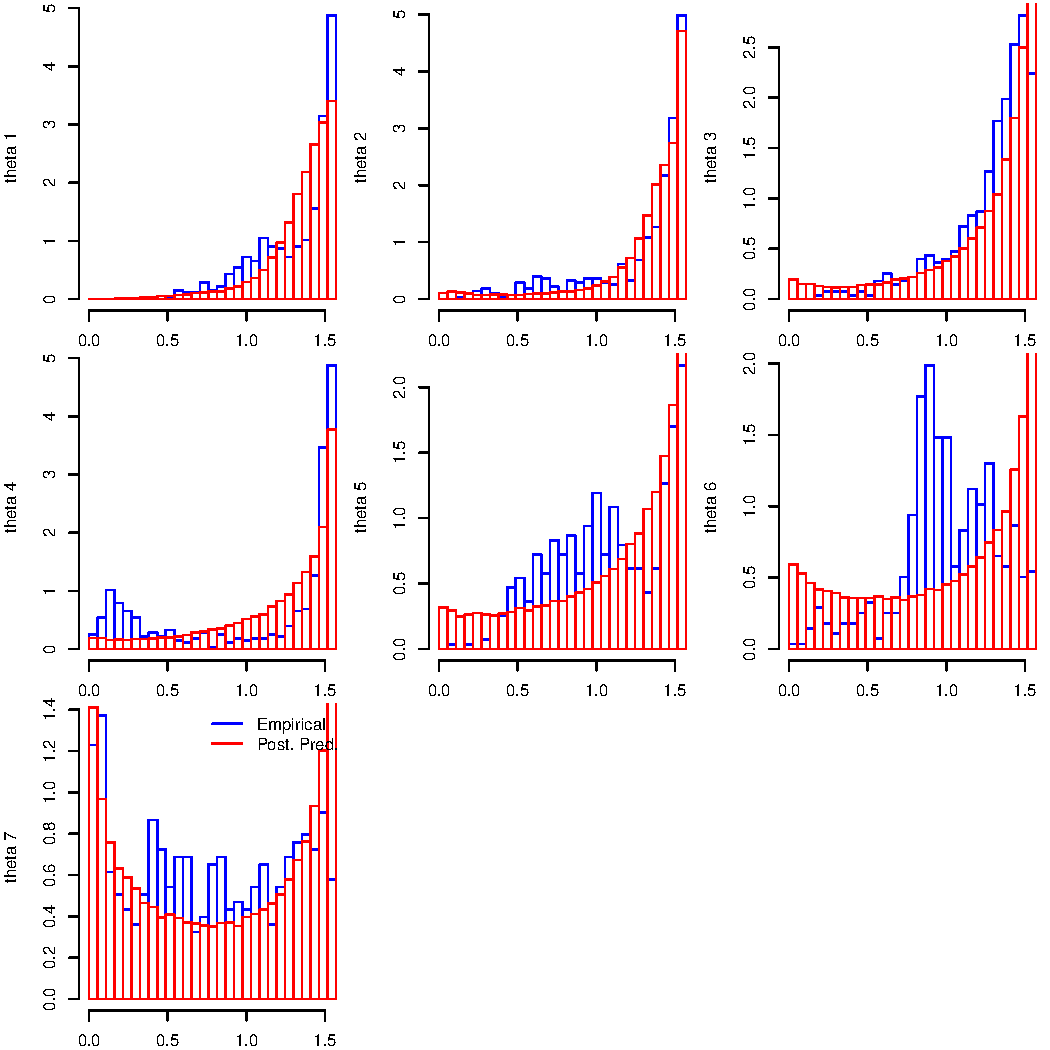
\includegraphics[width=6in]{./images/dpmpg_emp_v_pred_decluster}
\end{figure}

As it turns out, the model as specified above has issues with specifiability, resulting in model
  instability.  The course I took was to fit $b_{\alpha} = b_{\beta} = 1$.  This at least resulted
  in a stable model, but as we can see in Figure~\ref{fig:dpmpg}, the resulting distribution does
  not well match the original data.  The estimates for $a_{\alpha}$ (for all columns) are all
  between $0$ and $0.2$, while the estimates for $a_{\beta}$ (for all columns $> 1$) are stable
  around $20$.  This results, as a prior distribution for possible clusters, in each column having
  a very unstable distribution independent of other columns.  I believe this is why we see such a
  strong prior effect towards independence in Figure~\ref{fig:dpmpg}.

% EOF


\subsection{Spatial Threshold Modeling}
Following the work of \cite{ferreira2014}, any of the above methods can be
  extended to the spatial domain by modification of the marginalization process.
  Assume a spatial process $X({\bf s})$, ${\bf s}\in {\bf S}$.  Then take the
  transformation
\begin{equation}
  \label{eqn:spatial}
  Z({\bf s}) = \left(1 + \gamma({\bf s})\frac{X({\bf s}) - b_t({\bf s})}{a_t({\bf s})}\right)_{+}^{1/{\gamma({\bf s})}}
\end{equation}
  where $b_t({\bf s})$ is a function corresponding to a high threshold at location
  ${\bf s}$, analogous to the role $b_t$ played previously. $a_t({\bf s})$
  corresponds to a scaling function, and $\gamma({\bf s})$ an extremal value index
  function.







% EOF
